\section{Architektura serwera}\label{serwer:architektura}
Zważając na spostrzeżenia wynikające z rozdziału \ref{przygotowania:przypadki-uzycia}, zdecydowałem się na wydzielenie odpowiednich modułów w aplikacji serwerowej:
\begin{itemize}
    \item Moduł autoryzacji (ang. Auth)
    \item Moduł zadań (ang. Assignments)
    \item Moduł nauczyciela (ang. Teacher)
    \item Moduł ucznia (ang. Student)
\end{itemize}
Dodatkowo doszedłem do wniosku, że chciałbym móc łatwo wymieniać odpowiednie podmoduły w zależności od potrzeb.
Z tego powodu zdecydowałem się na wydzielenie zachowania, które będzie implementowane przez odpowiednie serwisy znajdujące się w modułach.
W czasie implementacji wydziliłem dodatkowo moduł pod nazwą \textit{Core}, który zawiera kontrakty definujące zachowanie serwisów.
Moduł ten jest wspólny dla wszystkich modułów i zawiera interfejsy, które muszą być zaimplementowane przez serwisy w modułach.
Dodatkowo zawiera on klasy służące do odwzorowania obiektów z bazy danych w postaci agnostycznej względem bazy danych oraz modułów.
Również w tym module umieściłem wspólne błędy, które są powszechnie używane w aplikacji(UserNotFoundException, AssignmentNotFoundException, itp.).
\begin{figure}[H]
    \centering
    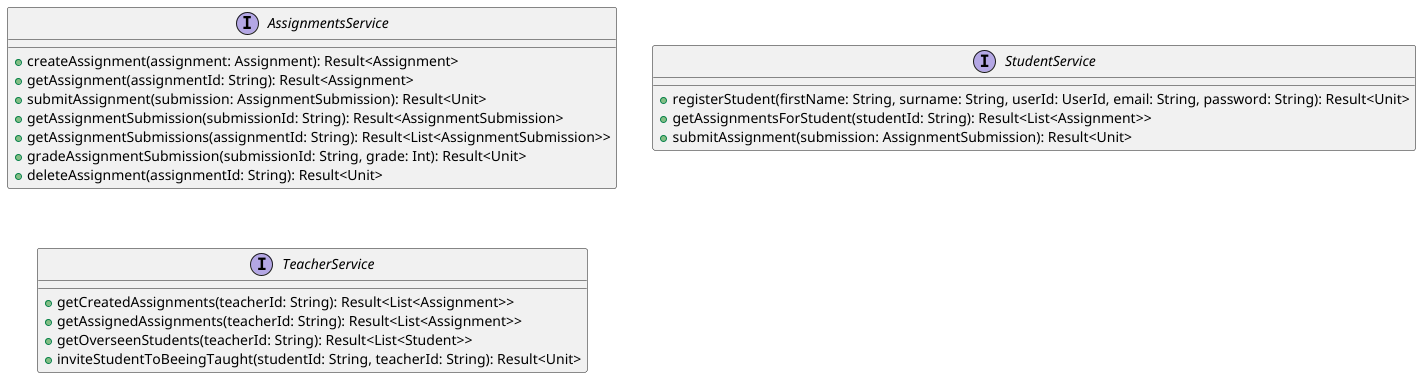
\includegraphics[width=15cm,keepaspectratio]{rysunki/adapters.png}
    \caption{Adaptery w aplikacji serwerowej}
    \label{fig:adapters}
\end{figure}

Na rysunku \ref{fig:adapters} przedstawiono schemat modułu \textit{Core} oraz interfejsów, które muszą być zaimplementowane przez serwisy w modułach.
Pozwala to na łatwe wymienianie serwisów w zależności od potrzeb.

